\section{Software Quality Metrics}
Citat fra Troels: \textit{''Hvad kan man finde ud af om sit program, uden at køre det? Denne disciplin kaldes Static Analysis, og kan give feedback til programmøren, der er ligeså værdifuld som en faktisk test.''}\\

Statisk analyse kan bruges til: 

\begin{enumerate}
	\item Give \textit{quality measures}.
	\item Gennemtvinge \textit{code style and discipline}.
	\item Finde \textit{possible errors}.
\end{enumerate}

\subsection{Værktøjer} 
Til formålet har vi nogle værktøjer. 

Da kode analyse kan tage lang tid, ligesom en langsom compilering, vil det ofte være en god ide at gøre det på en CI server.

\subsubsection{FxCop}
Statisk analyseværktøj, udviklet af Microsoft til Visual Studio. Lavet for at øge performance, sikkerhed og design.

\subsubsection{Compilers}
Compileren er et eksempel på et Statisk analyseværktøj. Alle moderne compilere viser advarseler og lignende for koden, nogle vigtige, andre - not so much. Intellisense i Visual Studio er et statisk analyseværktøj

\subsubsection{ReSharper}
Finder også fejl, som ikke nødvendigvis er kritiske. F.eks informerer den om inkonsekvent navngivning, ikke initialiserede variabler og helt ubrugte variabler.

\subsection{Statisk analyse}
Statisk analyse er en analyse af programmet uden at køre det.

\subsubsection{Kvantitativ analyse}
Aka: Software Metrics. Bruges til at beskrive: 
\begin{itemize}
	\item Microsoft Maintainability index.
	\item Cyclomatic complexity (se afsnit~\ref{sec:cyclomatic}).
	\item Lines of code per function/module.
\end{itemize}

\paragraph{MS Maintainability Index}
Et index som beskriver hvor holdbar og effektiv ens kode er. Samt hvor let den er at vedligeholde. Indexet går fra 0-100, hvor 100 er bedst.

\def\arraystretch{1.5}%  1 is the default, change whatever you need
\begin{table}[H]
	\centering
	\begin{tabular}{|c|l|}
		\hline
		\hspace{2cm} \cellcolor{green}& 20-100\\
		\hline
		\cellcolor{yellow}& 10-19\\
		\hline
		\cellcolor{red}& 0-9\\
		\hline
	\end{tabular}
	\caption{Maintainability index score.}
\end{table}

\paragraph{Lines of code}
Angiver antallet af \textit{intermediate language} linjer i koden, altså \textbf{ikke} linjer i source koden. Bruges til at indikere om en metode laver for meget og skal deles op i flere mindre methoder.

\paragraph{Class coupling}
En \textit{architectural} metric. Beskriver koblingen mellem klasser. Findes ved at kigge på parametre, returtyper, baseklasser, og interface-inplementeringer.

\paragraph{Depth of inheritance}
Angiver hvor mange klasser, der 'hænger' sammen i klassernes arveheiraki. Jo dybere et arveheiraki, desto svære at finde ud af hvor klasserne er defineret. Derved sværere at vedligeholde.

\paragraph{Cyclomatic Complexity}\label{sec:cyclomatic}
Bruges til at beskrive kompleksiteten i et program. Det er et kvantitativt mål for antallet af lineære uafhængige veje gemmen programmets source code.

Når man har en graf som vist på figur~\ref{fig:cyclomatic}, er følgende udtryk gældende: 

\begin{align}
E &= NumberOfEdges\\
N &= NumberOfNodes\\
P &= NumberOfConnectionComponents
\end{align}

\vskip.3cm

Med disse termer kan M (antallet af \textit{decision points}) findes sådan her:

\begin{align}
M &= E-N+2P\\
M&= 9-8+2*1=3
\end{align}

\begin{figure}[H]
	\centering
	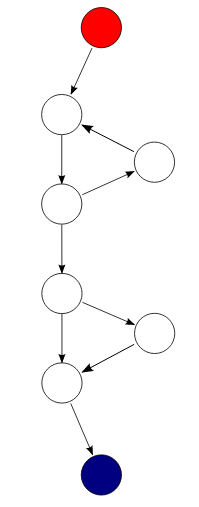
\includegraphics[width=0.8\linewidth]{figs/cyclomatic}
	\caption{Grafisk fremstiling af den cyclomatiske complexity i code listing~\ref{code:cyclomatic}.}
	\label{fig:cyclomatic}
\end{figure}

Ved software test er dette brugbart idet det giver et minimum for hvor mange testcases der er nødvendige for at få fuld test coverage.

For at forbedre sin cyklomatiske kompleksitet, kan man refaktuere sin kode til subfunctions og sub classes.

\begin{lstlisting}[caption=Kode for eksempel vist på figur~\ref{fig:cyclomatic}.,label=code:cyclomatic]
public void Method()
{
	while(Condition1) 
		Action1();		
	if(Condition2) 
		Action2();		
	Action3();	
	return;
}
\end{lstlisting}

\begin{figure}[H]
\centering
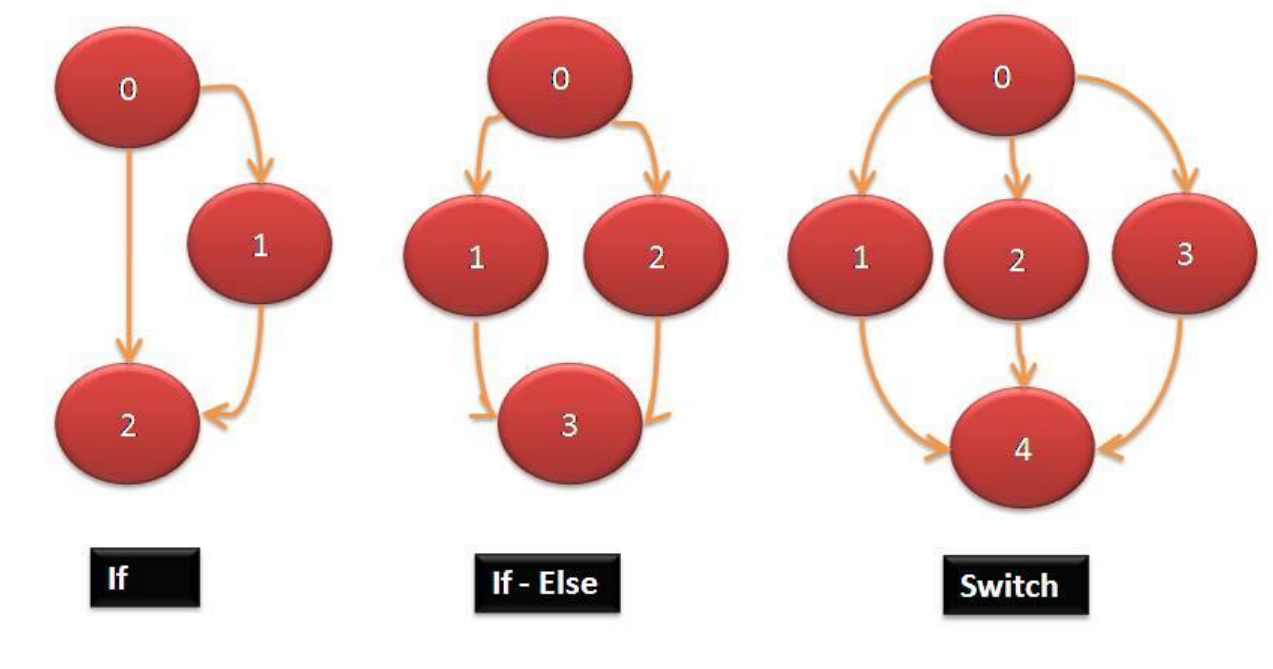
\includegraphics[width=0.8\linewidth]{figs/statementsgraph}
\caption{Tre forskellige statements som graf.}
\label{fig:statementsgraph}
\end{figure}


\subsubsection{Kvalitativ analyse}
Beskriver kodestil og -standard. Nogle fejl kan man reducere sig frem til, eksempelvis: 

\begin{itemize}
	\item Løse pointere.
	\item Memory leaks.
	\item Uinitialiserede variabler.
\end{itemize}

\subsection{Dynamisk analyse}
Til måling under kørsel af programmet. Bruges til at finde: 

\subsubsection{Kvalitative}

\begin{itemize}
	\item Unhandled exceptions.
	\item Index errors.
	\item Null pointers.
	\item Uninitialized variables.
	\item Writing outside allocated memory.
	\item Double deletes.
	\item Stack overflow
	\item ...
\end{itemize}

Når en af de førnævnte ting så finder sted kan følgende bruges til at konstatere nøjagtigt hvorfor:

\begin{itemize}
	\item Logging/tracing.
	\item Stack traces.
	\item Memory dumps.
	\item Monitoring/instrumentation.
\end{itemize}

Den nævnte instrumentering kan være \textit{Debug/Release}, \textit{Index check}, \textit{Assert(condition)} mm.

\subsubsection{Kvantitativ}
Målering af følgende attributter:

\begin{itemize}
	\item Time.
	\item CPU cycles.
	\item Memory footprint.
	\item OS resources.
	\item Memory leaks.
	\item Other bottlenecks (virtual memory vs. physical memory)
\end{itemize}

\subsection{Instrumented vs Sampled}
Der er flere værktøjer til opgaven, eksempelvis: VS Performance suite, Valgrind (Linux), Dmalloc (C og C++) og GNU gprof profiling. To forskellige måder at måde på:

\paragraph{Instrumented} very intrusive, high impact and precise.

\begin{enumerate}
	\item Compileren indsætter code for at måle. I hver function og linje.
	\item Programmet køres og data indsamles.
	\item Indsamlet data rapporteres.
\end{enumerate}

\paragraph{Sampled} not intrusive, small impact and medium precise.

\begin{enumerate}
	\item Compileren genererer et slags 'codemap' for source koden.
	\item Programmet køres og data indsamles på bestemte tidspunkter.
	\item Data rapporteres.
\end{enumerate}

Denne slags analyse er en god kandidat for CI. Lange og tunge byg kan fordelagtigt køres om natten som et \textit{nightly build}.

\begin{figure}[H]
\centering
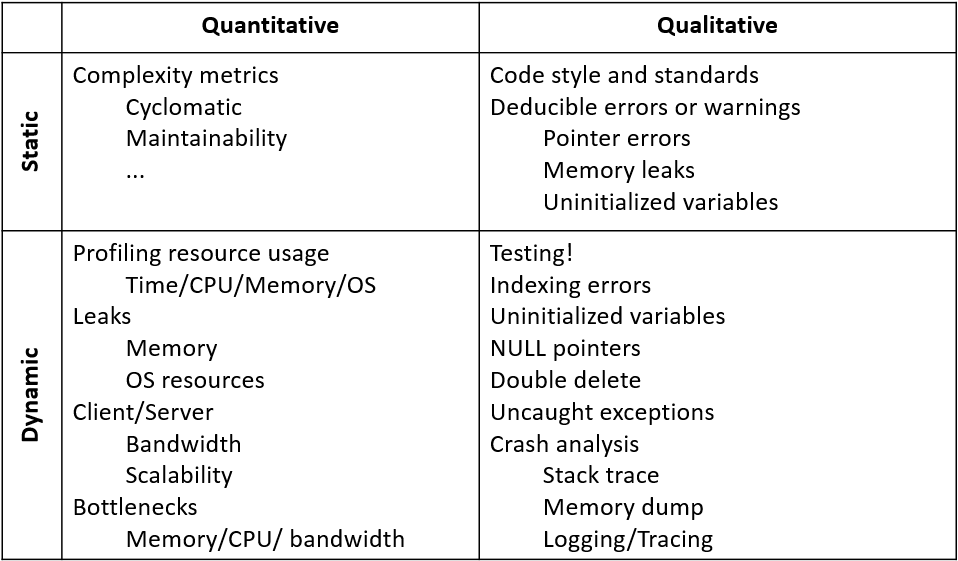
\includegraphics[width=\linewidth]{figs/static_dynamic}
\caption{Statisk vs. Dynamisk analyse.}
\label{fig:staticdynamic}
\end{figure}






